\documentclass[tikz,border=6pt]{standalone}
\usepackage{amsmath,amssymb,mathtools,physics,bm,nicefrac,wasysym}
\usepackage{xcolor}

\definecolor{colone}{RGB}{180,60,60}
\definecolor{coltwo}{RGB}{60,110,180}
\definecolor{colthree}{RGB}{60,140,80}

\definecolor{accent}{HTML}{A13D2C}
\definecolor{accent2}{HTML}{2B5F6B}
\definecolor{muted}{HTML}{5A564F}
\definecolor{panel}{HTML}{F8F6F0}
\definecolor{linecol}{HTML}{D8D2C4}
\definecolor{ink}{HTML}{1E1C1A}
\definecolor{astroblue}{HTML}{1B4F72}
\definecolor{astrodark}{HTML}{17202A}
\definecolor{sunyellow}{HTML}{E8A33D}

\usetikzlibrary{calc,arrows.meta,positioning,decorations.pathreplacing,decorations.markings,angles,quotes,shapes.geometric}
\usepackage{tikz-3dplot}

\newcommand{\vecr}{\vec r}
\newcommand{\vecL}{\vec L}
\newcommand{\vecA}{\vec A}
\newcommand{\vecf}{\vec f}
\newcommand{\vecF}{\vec F}
\newcommand{\vecp}{\vec p}
\newcommand{\avg}[1]{\left\langle #1\right\rangle}
\newcommand{\vecx}{\vec x}
\newcommand{\hatn}{\hat n}
\newcommand{\rhat}{\hat r}
\newcommand{\phihat}{\hat\phi}
\newcommand{\thetahat}{\hat\theta}
\newcommand{\note}[1]{\textcolor{blue!60!black}{\textit{[#1]}}}

\newcommand{\LST}{\mathrm{LST}}
\newcommand{\GST}{\mathrm{GST}}
\newcommand{\GMST}{\mathrm{GMST}}
\newcommand{\GAST}{\mathrm{GAST}}
\newcommand{\LMST}{\mathrm{LMST}}
\newcommand{\LAST}{\mathrm{LAST}}
\newcommand{\UT}{\mathrm{UT}}
\newcommand{\UTC}{\mathrm{UTC}}
\newcommand{\TAI}{\mathrm{TAI}}
\newcommand{\TT}{\mathrm{TT}}
\newcommand{\TDB}{\mathrm{TDB}}
\newcommand{\JD}{\mathrm{JD}}
\newcommand{\MJD}{\mathrm{MJD}}
\newcommand{\EoT}{\mathrm{EoT}}
\newcommand{\SNR}{\mathrm{SNR}}
\newcommand{\RON}{\mathrm{RON}}



\begin{document}
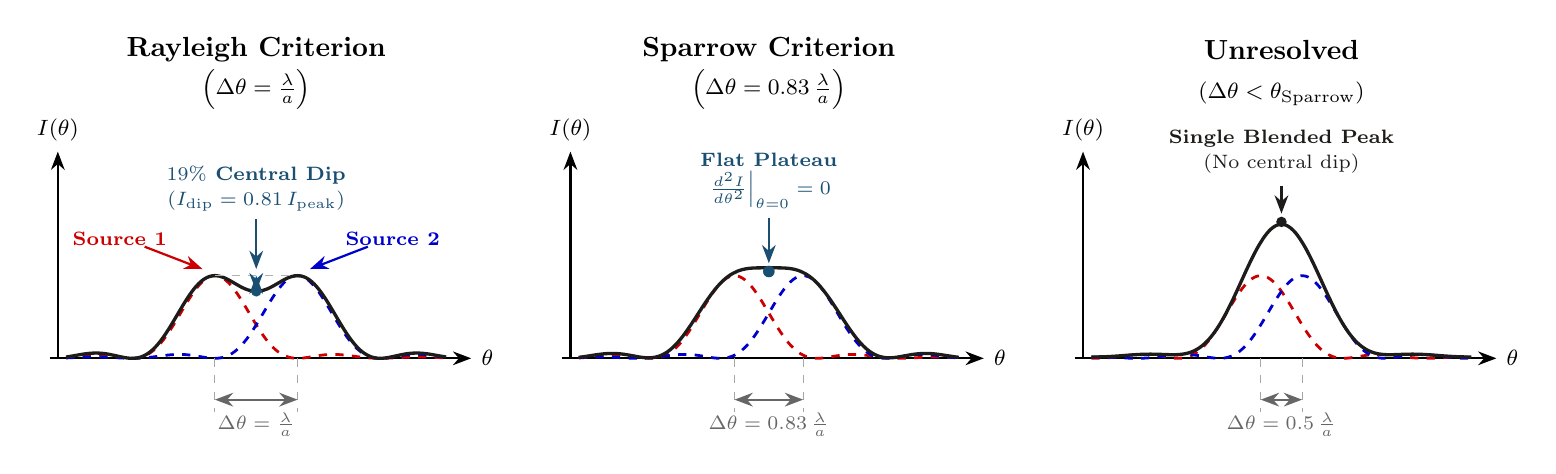
\begin{tikzpicture}[
    scale=1.05, 
    >=Stealth,
    declare function={
        sinc(\x) = (\x==0 ? 1.0 : sin(deg(\x))/\x);
        psf1(\x,\sep) = pow(sinc(3.14159*(\x + 0.5*\sep)), 2);
        psf2(\x,\sep) = pow(sinc(3.14159*(\x - 0.5*\sep)), 2);
        psftot(\x,\sep) = psf1(\x,\sep) + psf2(\x,\sep);
    }
]
    % 1. Rayleigh Criterion (\sep = 1.0)
    \begin{scope}[shift={(0,0)}]
        \def\sep{1.0}
        \node[font=\bfseries\normalsize, align=center] at (0, 3.45) {Rayleigh Criterion\\[2pt]\footnotesize\mdseries $\left(\Delta\theta = \frac{\lambda}{a}\right)$};
        
        \draw[->, thick] (-2.5, 0) -- (2.6, 0) node[right, font=\footnotesize] {$\theta$};
        \draw[->, thick] (-2.4, 0) -- (-2.4, 2.5) node[above, font=\footnotesize] {$I(\theta)$};
        
        \draw[dashed, red!80!black, line width=1.0pt, domain=-2.3:2.3, samples=150] plot (\x, {psf1(\x,\sep)});
        \draw[dashed, blue!80!black, line width=1.0pt, domain=-2.3:2.3, samples=150] plot (\x, {psf2(\x,\sep)});
        \draw[very thick, ink, domain=-2.3:2.3, samples=200] plot (\x, {psftot(\x,\sep)});
        
        \node[font=\scriptsize\bfseries, red!80!black, align=center] at (-1.65, 1.45) {Source 1};
        \draw[->, thick, red!80!black] (-1.35, 1.35) -- (-0.65, 1.08);
        
        \node[font=\scriptsize\bfseries, blue!80!black, align=center] at (1.65, 1.45) {Source 2};
        \draw[->, thick, blue!80!black] (1.35, 1.35) -- (0.65, 1.08);
        
        \draw[dashed, gray!60, thin] (-0.5, 1.0) -- (0.5, 1.0);
        \draw[<->, thick, astroblue] (0, 0.81) -- (0, 1.0);
        \node[font=\scriptsize\bfseries, astroblue, align=center] at (0, 2.05) {$19\%$ Central Dip\\[1pt]\mdseries ($I_{\rm dip} = 0.81\,I_{\rm peak}$)};
        \draw[->, thick, astroblue] (0, 1.68) -- (0, 1.08);
        \fill[astroblue] (0, 0.81) circle (1.8pt);
        
        \draw[dashed, gray!70] (-0.5, 0) -- (-0.5, -0.65);
        \draw[dashed, gray!70] (0.5, 0) -- (0.5, -0.65);
        \draw[<->, thick, gray!80!black] (-0.5, -0.5) -- (0.5, -0.5) 
            node[midway, below=1pt, font=\scriptsize\bfseries] {$\Delta\theta = \frac{\lambda}{a}$};
    \end{scope}

    % 2. Sparrow Criterion (\sep = 0.83)
    \begin{scope}[shift={(6.2,0)}]
        \def\sep{0.83}
        \node[font=\bfseries\normalsize, align=center] at (0, 3.45) {Sparrow Criterion\\[2pt]\footnotesize\mdseries $\left(\Delta\theta = 0.83\,\frac{\lambda}{a}\right)$};
        
        \draw[->, thick] (-2.5, 0) -- (2.6, 0) node[right, font=\footnotesize] {$\theta$};
        \draw[->, thick] (-2.4, 0) -- (-2.4, 2.5) node[above, font=\footnotesize] {$I(\theta)$};
        
        \draw[dashed, red!80!black, line width=1.0pt, domain=-2.3:2.3, samples=150] plot (\x, {psf1(\x,\sep)});
        \draw[dashed, blue!80!black, line width=1.0pt, domain=-2.3:2.3, samples=150] plot (\x, {psf2(\x,\sep)});
        \draw[very thick, ink, domain=-2.3:2.3, samples=200] plot (\x, {psftot(\x,\sep)});
        
        \node[font=\scriptsize\bfseries, astroblue, align=center] at (0, 2.15) {Flat Plateau\\[1pt]\mdseries $\left.\frac{d^2 I}{d\theta^2}\right|_{\theta=0} = 0$};
        \draw[->, thick, astroblue] (0, 1.70) -- (0, 1.15);
        \fill[astroblue] (0, 1.05) circle (2pt);
        
        \draw[dashed, gray!70] (-0.415, 0) -- (-0.415, -0.65);
        \draw[dashed, gray!70] (0.415, 0) -- (0.415, -0.65);
        \draw[<->, thick, gray!80!black] (-0.415, -0.5) -- (0.415, -0.5) 
            node[midway, below=1pt, font=\scriptsize\bfseries] {$\Delta\theta = 0.83\,\frac{\lambda}{a}$};
    \end{scope}

    % 3. Unresolved (\sep = 0.50)
    \begin{scope}[shift={(12.4,0)}]
        \def\sep{0.50}
        \node[font=\bfseries\normalsize, align=center] at (0, 3.45) {Unresolved\\[2pt]\footnotesize\mdseries $(\Delta\theta < \theta_{\rm Sparrow})$};
        
        \draw[->, thick] (-2.5, 0) -- (2.6, 0) node[right, font=\footnotesize] {$\theta$};
        \draw[->, thick] (-2.4, 0) -- (-2.4, 2.5) node[above, font=\footnotesize] {$I(\theta)$};
        
        \draw[dashed, red!80!black, line width=1.0pt, domain=-2.3:2.3, samples=150] plot (\x, {psf1(\x,\sep)});
        \draw[dashed, blue!80!black, line width=1.0pt, domain=-2.3:2.3, samples=150] plot (\x, {psf2(\x,\sep)});
        \draw[very thick, ink, domain=-2.3:2.3, samples=200] plot (\x, {psftot(\x,\sep)});
        
        \node[font=\scriptsize\bfseries, ink, align=center] at (0, 2.50) {Single Blended Peak\\[1pt]\mdseries (No central dip)};
        \draw[->, thick, ink] (0, 2.08) -- (0, 1.75);
        \fill[ink] (0, 1.65) circle (1.8pt);
        
        \draw[dashed, gray!70] (-0.25, 0) -- (-0.25, -0.65);
        \draw[dashed, gray!70] (0.25, 0) -- (0.25, -0.65);
        \draw[<->, thick, gray!80!black] (-0.25, -0.5) -- (0.25, -0.5) 
            node[midway, below=1pt, font=\scriptsize\bfseries] {$\Delta\theta = 0.5\,\frac{\lambda}{a}$};
    \end{scope}
\end{tikzpicture}
\end{document}
